\section{MSL Use-Case Examples}

As an example, we will illustrate the commands required to set up and
run a filter on a single core. For simplicity, we assume the filter is
connected to a buffer that provides a FIFO abstraction over tapes (the
input buffer is the input tape, and the output buffer is the output
tape). The filter has a single input tape, single output tape, and
static rates: its work function pops $i$, peeks $i+e$, and pushes $o$
bytes per iteration.

Before the filter can be run, it must be loaded, its input and output
buffers must be allocated, and the filter's tapes must be attached to the
buffers. The commands that perform this are illustrated in
Figure~\ref{fig:lib:init}.

\begin{figure}[!htb]
\begin{center}
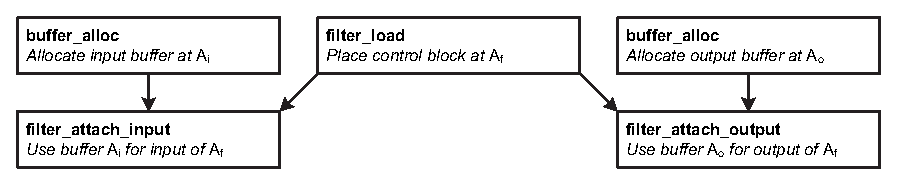
\includegraphics[scale=.55]{figs/init-efont}
\end{center}
\caption[Commands to set up a filter.]{Commands to load a filter and to allocate and attach input and output buffers. Lines between commands represent dependencies that must be specified to the library when the commands are issued. These commands may be issued in one or multiple groups.}
\label{fig:lib:init}
\end{figure}

In addition, input data must be transferred into the input buffer before the filter can be run, and output data must eventually be transferred out of the output buffer. With an initially empty input buffer, the commands to transfer in $n$ iterations of input, run the filter for $n$ iterations, and then transfer out $n$ iterations of output (assuming that the input and output buffers were sized appropriately) are shown in Figure~\ref{fig:lib:run}.

\begin{figure}[!htb]
\begin{center}
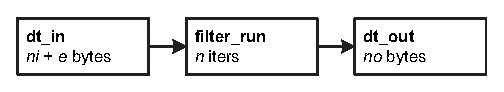
\includegraphics{figs/run-efont}
\end{center}
\caption[Commands to run a filter.]{Commands to run a filter for the
  first $n$ iterations, including transferring input and output. The
  corresponding data transfer commands on other cores are not shown.}
\label{fig:lib:run}
\end{figure}

A sequence of commands is required to run the filter for a larger
number of iterations on a core with a finite local store
capacity. This is illustrated in Figure~\ref{fig:lib:ext}.

\begin{figure}[!htb]
\begin{center}
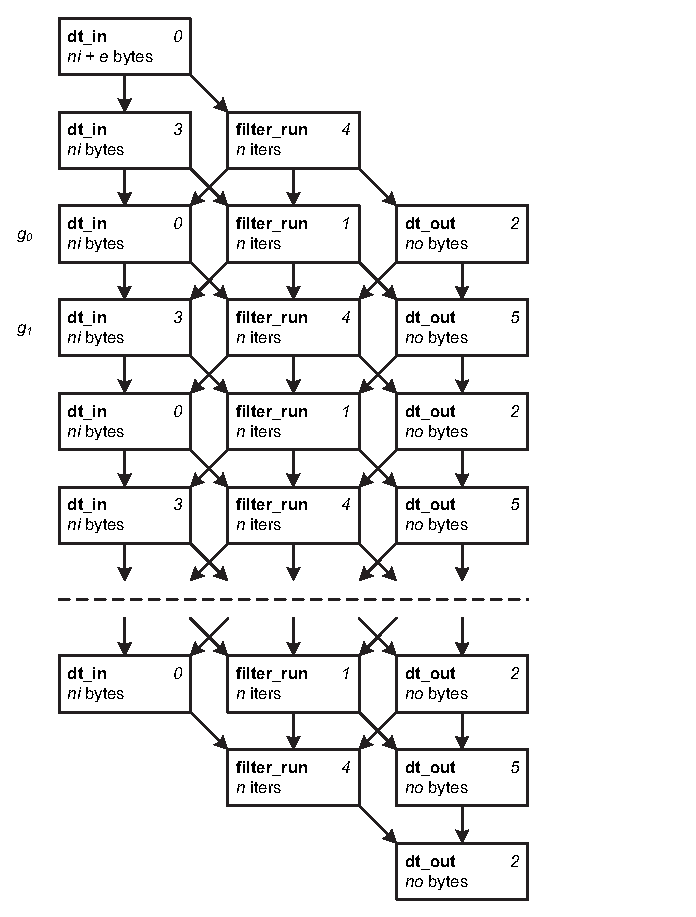
\includegraphics[scale=.90]{figs/ext-efont}
\end{center}
\caption[Sequence of commands to run a filter for a large number of iterations.]{Sequence of commands to run a filter for a large number of iterations. Command IDs are indicated in the upper right. Each row is issued as a different group.}
\label{fig:lib:ext}
\end{figure}

Provided that the input buffer is at least $2ni+e$ bytes and the output buffer is at least $2no$ bytes, the dependencies among the commands in the sequence ensure that:
\begin{itemize}
\item When a \textsf{dt\_in} command becomes active, there are at most $ni+e$ bytes of data in the input buffer, and thus enough space to transfer in an additional $ni$ bytes.
\item When a \textsf{dt\_out} command becomes active, there are at least $no$ bytes of data in the output buffer, and thus enough data to transfer out.
\item When a \textsf{filter\_run} command becomes active, there are at least $ni+e$ bytes of data in the input buffer and at most $no$ bytes of data in the output buffer. This is enough input data and output space to run the filter for $n$ iterations.
\end{itemize}

This sequence of commands effectively ``pipelines'' the basic operation from Figure~\ref{fig:lib:run}. Double-buffering is accomplished when the data transfer commands in a group complete before the \textsf{filter\_run} does. In this case, the following \textsf{filter\_run} has no outstanding dependencies once the current \textsf{filter\_run} completes, and can become active immediately.

The user or scheduler can keep the core continually supplied with work
by initially issuing the first two groups and thereafter issuing the next
group whenever a group completes. In this case, the core almost always
has two groups of commands issued, with one group active and the other
queued. In addition, with the exception of the first two and last two
groups, the command parameters, IDs and dependencies in every other
group are identical. This allows the user to initially set up two
groups ($g_0$ and $g_1$ in Figure~\ref{fig:lib:ext}) and repeatedly
issue them for a majority of the execution. If executions are
relatively long, the overhead of the first and last group, where no
filter is being run, will be amortized effectively. Alternatively, the
user can load another filter and run it during those gaps.

In practice, situations such as the above, where a static-rate filter
is run for a large number of iterations and large amounts of input and
output data are transferred, are very common in streaming applications. To
avoid requiring the user to manually issue groups and deal with
command completion callbacks in every such case, the MSL library also
provides extended operations that encapsulate this pattern. In an
extended operation, the user provides the library with filter rates,
the addresses of opposing buffers on other processors for data
transfers, and the number of iterations to run for; the library issues and
responds to all commands internally and notifies the user when the
entire operation is complete.
%% Where one or both opposing buffers are located in memory,
%% the library also handles the PPE side of data transfers
%% internally. 
Extended operations greatly simplify setting up pipelines
of any length where all filters in the pipeline have static rates.

